\documentclass[a4paper, 12pt]{article}
\usepackage[a4paper,top=1.5cm, bottom=1.5cm, left=1cm, right=1cm]{geometry}
\usepackage{cmap}					
\usepackage{mathtext} 				
\usepackage[T2A]{fontenc}			
\usepackage[utf8]{inputenc}			
\usepackage[english,russian]{babel}
\usepackage{multirow}
\usepackage{graphicx}
\usepackage{wrapfig}
\usepackage{tabularx}
\usepackage{float}
\usepackage{longtable}
\usepackage{hyperref}
\hypersetup{colorlinks=true,urlcolor=blue}
\usepackage[rgb]{xcolor}
\usepackage{amsmath,amsfonts,amssymb,amsthm,mathtools} 
\usepackage{icomma} 
\usepackage{euscript}
\usepackage{mathrsfs}
\usepackage{enumerate}
\usepackage{caption}
\usepackage{enumerate}
\mathtoolsset{showonlyrefs=true}
\usepackage{graphicx}
\usepackage{caption}
\usepackage{subcaption}
\usepackage[europeanresistors, americaninductors]{circuitikz}
\DeclareMathOperator{\sgn}{\mathop{sgn}}
\newcommand*{\hm}[1]{#1\nobreak\discretionary{}
	{\hbox{$\mathsurround=0pt #1$}}{}}

\title{\textbf{Изучение вынужденной регулярной прецессии гироскопа (1.2.5)}}
\author{Манро Эйден}
\date{}

\begin{document}

\maketitle
	      	
    \begin{center}
    \section*{Введение}    
    \end{center}

    \noindent \textbf{Цель работы:} исследовать вынужденную прецессию гироскопа; установить зависимость скорости вынужденной прецессии от величины момента сил, действующих на ось гироскопа; определить скорость вращения ротора гироскопа и сравнить ее со скоростью, рассчитанной по скорости прецессии.

    \bigskip

    \noindent \textbf{Оборудование:} гироскоп в кардановом подвесе, секундомер, набор грузов, отдельный ротор гироскопа, цилиндр известной массы, крутильный маятник, штангенциркуль, линейка, осцилограф, генератор частоты.
    
    \bigskip
    \begin{center}
        \subsection*{Теоретические сведения}
        Уравнение движения твёрдого тела можно записать в следующем виде:

\begin{equation}
\frac{d\vec{P}}{dt}=\vec{F}
\label{one}
\end{equation}

\begin{equation}
\frac{d\vec{L}}{dt}=\vec{M}
\label{two}
\end{equation}

Момент импульса тела в главных его осях $x$, $y$, $z$ равен

\begin{equation}
\vec{L} = \vec{i}I_x\omega_x+\vec{j}I_y\omega_y+\vec{k}I_z\omega_z,
\label{three}
\end{equation}
где $ I_x $, $ I_y $, $ I_z $ -- главные моменты инерции, $ \omega_x $, $ \omega_y $, $ \omega_z $ -- компоненты вектора угловой скорости $ \vec{\omega} $. Быстро вращающееся тело, для которого, например,

\begin{equation}
I_z\omega_z \gg I_x\omega_x,\;\;\;\;I_y\omega_y,
\end{equation} 
принято называть гироскопом. Гироскоп называется уравновешенным, если его центр масс неподвижен.

В силу \eqref{two} приращение момента импульса определяется интегралом

\begin{equation}
\Delta\vec{L} = \int\vec{M} dt.
\label{four}
\end{equation}
Если момент внешних сил действует в течение короткого промежутка времени, из интеграла \eqref{four} следует, что приращение $ \Delta \vec{L} $ момента импульса значительно меньше самого момента импульса:

\begin{equation}
\left|\Delta \vec{L}\right| \ll \left|\vec{L}\right| 
\end{equation}

С этим связана замечательная устойчивость, которую приобретает движение гироскопа после приведения его в быстрое вращение. 
Выясним, какие силы надо приложить к гироскопу, чтобы изменить 
направление его оси. Рассмотрим для 
примера маховик, вращающийся вокруг оси $ z $, перпендикулярной к плоскости маховика (рис. \ref{mahovik}). Будем считать, что

\begin{equation}
\omega_z = \omega_0, \;\;\;\;\; \omega_x = 0, \;\;\;\;\; \omega_y = 0.
\end{equation}

\noindent Пусть ось вращения повернулась в плоскости $ zx $ по направлению к оси $ x $ на бесконечно малый угол $ d\varphi $. Такой поворот означает добавочное вращение маховика вокруг оси $ y $, так что

\begin{equation}
d\varphi=\Omega dt,
\end{equation}
где $ \Omega $ -- угловая скорость такого вращения. Будем предполагать, что

\begin{equation}
L_\Omega \ll L_{\omega_0}
\label{five}
\end{equation}
Это означает, что момент импульса маховика, равный $ I_z\omega_0 $ до приложения внешних сил, только повернётся в плоскости $ zx $ по направлению к оси $ x $, не изменяя своей величины. Таким образом, 

\begin{equation}
\left|d\vec{L}\right| = Ld\varphi = L\Omega dt.
\end{equation}
Но это изменение направлено вдоль оси $ x $, поэтому вектор $ d\vec{L} $ можно представить в виде векторного произведения вектора угловой скорости $ \omega $, направленного вдоль оси $ y $, на вектор собственного момента импульса маховика, направленного вдоль оси $ z $,

\begin{equation}
d\vec{L}=\vec{\Omega} \times \vec{L} dt,
\end{equation}
т. е.

\begin{equation}
\frac{d\vec{L}}{dt} = \vec{\Omega} \times \vec{L}.
\end{equation}
В силу \eqref{two} имеем

\begin{equation}
\vec{M} = \vec{\Omega} \times \vec{L}.
\label{six}
\end{equation}
Формула \eqref{six} справедлива, если выполнено условие \eqref{five}. Она позволяет определить момент сил $ \vec{M} $, который необходимо приложить к маховику для того, чтобы вызвать вращение оси маховика с угловой скоростью $ \vec{\Omega} $. Мы видим, таким образом, что для поворота оси вращающегося маховика к оси $ x $ необходимо приложить силы, направленные не вдоль оси $ x $, а вдоль оси $ y $, так чтобы их момент $ \vec{M} $ был направлен вдоль оси $ x $.

Для гироскопа массой $ m_\text{г} $, у которого ось собственного вращения наклонена на угол $ \alpha $ от вертикали, скорость прецессии, происходящей вокруг вертикальной оси под действием силы тяжести, равна

\begin{equation}
\Omega = \frac{M}{I_z\omega_0\sin \alpha} = \frac{m_\text{г}gl_\text{ц}\sin\alpha}{I_z\omega_0\sin\alpha} = \frac{m_\text{г}gl_\text{ц}}{I_z\omega_0},
\end{equation}
где $ l_\text{ц} $ -- растояние от точки подвеса до центра масс гироскопа, т. е. скорость прецессии не зависит от угла $ \alpha $.

Для изучения регулярной прецессии уравновешенного гироскопа к его оси подвешивают дополнительные грузы. Это смещает общий центр масс и создает момент сил тяжести, вызывающий прецессию. Скорость прецессии в этом случае равна

\begin{equation}
\Omega = \frac{mgl}{I_z\omega_0},
\label{eight}
\end{equation}
где $ m $ -- масса груза, $ l $ -- расстояние от центра карданова подвеса до точки крепления груза на оси гироскопа.

Измерение скорости прецессии гироскопа позволяет вычислить угловую скорость вращения его ротора. Расчет производится по формуле \eqref{eight}. Момент инерции ротора относительно оси симметрии $ I_0 $ измеряется по крутильным колебаниям точной копии ротора, подвешиваемой вдоль оси симметрии на жесткой проволоке. Период крутильных колебаний $ T_0 $ зависит от момента инерции $ I_0 $ и модуля кручения проволоки $ f $:

    \begin{equation}
        T_0 = 2\pi\sqrt{\frac{I_0}{f}}.
        \label{nine}
    \end{equation}


    \begin{figure}
    	\centering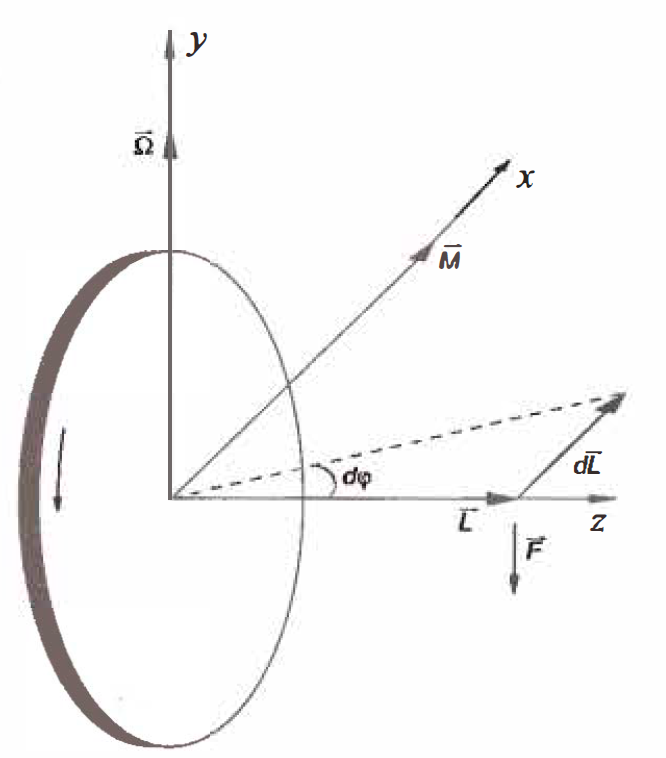
\includegraphics[width=8cm]{mahovik.png}
    	\caption{Маховик}
    	\label{mahovik}
    \end{figure}
    
Чтобы исключить модуль кручения проволоки, вместо ротора гироскопа к той же проволоке подвешивают цилиндр правильной формы с известными размерами и массой, для которого легко можно вычислить момент инерции $ I_\text{ц} $. Для определения момента инерции ротора гироскопа имеем 

    \begin{equation}
        I_0=I_\text{ц}\frac{T_0^2}{T_\text{ц}^2},
        \label{ten}
    \end{equation}


\bigskip

где $ T_\text{ц} $ - период крутильных колебаний цилиндра.
\end{center}

    \subsection*{\centering Экспериментальная установка}   

\bigskip

    \begin{figure}[H]
    	\centering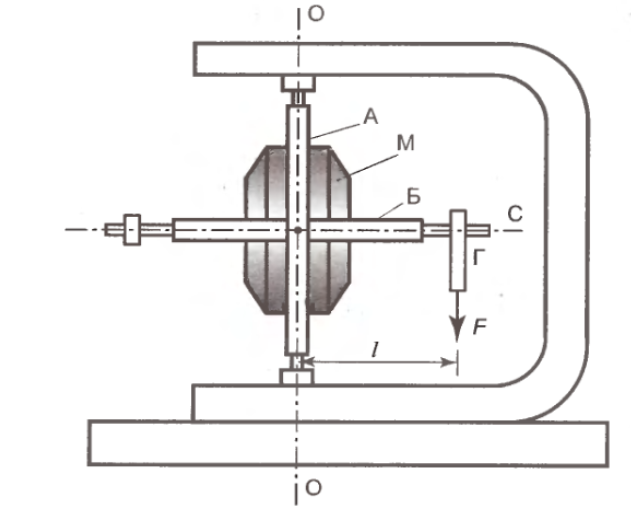
\includegraphics[width=10cm]{ustanovka.png}
    	\caption{Схема экспериментальной установки}
    	\label{ustanovka}
    \end{figure}

\newpage
\begin{center}
\subsection*{Погрешности}

    \begin{itemize}
	\item \textbf{Линейка:} $ \Delta_\text{лин} = 0,001 $ м
	\item \textbf{Секундомер:} $ \Delta_\text{сек} = 0,5 $ с \text{(с учётом реакции человека)}
	\item \textbf{Электронные весы:} $ \Delta_\text{вес} = 0,001 $ кг
\end{itemize}

\end{center}

\begin{center}
    \section*{Ход работы}

    Для определения момента инерции цилиндра по формуле \eqref{ten} необходимо измерить период крутильных колебаний пробного цилиндра известной массы, вычислить его момент инерции и измерить период крутильных колебаний ротора гироскопа на той же проволоке.
    \bigskip

    Момент инерции цилиндра можно вычислить по следующей формуле:

    \begin{equation}
        I_\text{ц} = \frac{1}{2}m_\text{ц}\left( \frac{d_\text{ц}}{2}\right)^2,
    \end{equation}
    
    где $ m_\text{ц} $ -- масса цилиндра, $ d_\text{ц} $ -- его диаметр.
    \bigskip

    При измерении этих параметров получаем:
	 $ m_\text{ц} = \left( 1,616 \pm 0,001\right) $ кг,
      $ d_\text{ц} = \left( 0,078 \pm 0,001 \right) $ м

    \bigskip
    Тогда
    \begin{equation}
        I_\text{ц} = 1,22 \cdot 10^{-3} \text{ кг} \cdot \text{м}^2
    \end{equation}

    Погрешность вычисления момента инерции цилиндра может быть найдена по следующей формуле:

    \begin{equation}
        \sigma_{I_\text{ц}} = I_\text{ц}\sqrt{\left( \frac{\Delta_\text{вес}}{m_\text{ц}} \right)^2 + \left(2 \frac{\Delta_\text{лин}}{d_\text{ц}} \right)^2 } \approx 3 \cdot 10^{-5} \text{ кг} \cdot \text{м}^2
    \end{equation}

    В итоге:
    \bigskip
    
    \underline{$ I_\text{ц} = \left(0,00122 \pm 0,00003 \right) \text{ кг} \cdot \text{м}^2 $, $ \left( \varepsilon = 2,4 \% \right) $}

    \bigskip \bigskip

    Производим измерение времени 10 крутильных колебаний цилиндра. Полученные результаты заносим в таблицу \ref{krut_cil}.
    \bigskip

    \begin{table}[H]
    	\centering
    	\begin{tabular}{|c|c|c|c|}
    		                                                       \hline
    		$ t $, с & $ N $ & $ T $, с & $ \sigma_T $, с      \\ \hline
                39,41    &   10  &  3,94    & 0,5                  \\ \hline
    	\end{tabular}
    	\caption{Результат измерения периода крутильных колебаний цилиндра}
    	\label{krut_cil}
    \end{table}

    \label{formuli}

    Период колебаний может быть рассчитан по формуле:
    \begin{equation}
        T = \frac{t}{N}.
    \end{equation}


    В итоге: 
    \bigskip

    \underline{$ T_\text{ц} = \left( 3,94 \pm 0,05\right) $ с, $ \left(\varepsilon = 1,2 \% \right)  $}

    \newpage

    Аналогично измерим период крутильных колебаний ротора гироскопа.

    \bigskip

    \begin{table}[H]
    	\centering
    	\begin{tabular}{|c|c|c|c|}
    		                                                       \hline
    		$ t $, с & $ N $ & $ T $, с & $ \sigma_T $, с      \\ \hline
                31,25    &   10  &  3,13    & 0,5                  \\ \hline
    	\end{tabular}
    	\caption{Результат измерения периода крутильных колебаний ротора гироскопа}
    	\label{krut_gil}
    \end{table}

     В итоге: 
    \bigskip

    \underline{$ T_\text{ц} = \left( 3,13 \pm 0,05\right) $ с, $ \left(\varepsilon = 1,5 \% \right)  $}

    \bigskip
    
    По формуле \eqref{ten} вычислим момент инерции ротора гироскопа:

    \begin{equation}
        I_0=I_\text{ц}\frac{T_0^2}{T_\text{ц}^2} = 0,00077 \text{ кг} \cdot \text{м}^2.
    \end{equation}

Погрешность вычисления момента инерции ротора гироскопа можно вычислить по формуле:

    \begin{equation}
        \sigma_{I_0} = I_0\sqrt{\left( \varepsilon_{I_\text{ц}} \right)^2 +\left( 2 \varepsilon_{T_0} \right)^2 + \left(2 \varepsilon_{T_\text{ц}} \right)^2} \approx 0,00003 \text{ кг} \cdot \text{м}^2.
    \end{equation}

В итоге:

\bigskip

\underline{$ I_0 = \left( 0,00077 \pm 0,00003 \right) \text{ кг} \cdot \text{м}^2, \left( \varepsilon = 3,9   \% \right) $}

\bigskip \bigskip

Для определения частоты вращения ротора гироскопа будем исследовать зависимость скорости прецессии гироскопа в зависимости от момента силы, действующей на его ось. Результаты измерений представлены в таблице \ref{sk_pre}.

    \begin{table}[H]
    	\centering
    	\begin{tabular}{|c|c|c|c|c|c|c|c|c|c|c|c|}
                \hline
		№  & $ m $, кг          & $ l $, м            & $ M $, Н$\cdot$м      & $ \sigma_M $, Н$\cdot$м             & $ t $, с & $ N$ & $ T $, с  & $ \sigma_T $, с          &  $ \varepsilon_T, \%$   & $ \Omega $, $ \text{с}^{-1} $ & $ \sigma_\Omega $, $ \text{с}^{-1} $ \\ \hline
  
        1 & 0,074 & 0,122 &  0,089 & 0,001  & 139,48 & 1 & 139,48 & 0,5 & 0,3 & 0,045 & 0,001 \\ \hline

        2 & 0,092 & 0,122 &  0,109 & 0,001  & 110,54 & 1 & 110,54 & 0,5 & 0,4 & 0,056 & 0,001 \\ \hline

        3 & 0,116 & 0,122 &  0,138 & 0,002  & 88,06  & 1 & 88,06 & 0,5 & 0,5 & 0,071 & 0,001 \\ \hline

        4 & 0,141 & 0,122 &  0,169 & 0,002  & 72,22  & 1 & 72,22 & 0,5 & 0,6 & 0,087 & 0,001 \\ \hline

        5 & 0,179 & 0,122 &  0,214 & 0,002  & 59,91  & 1 & 59,91 & 0,5 & 0,8 & 0,104 & 0,001 \\ \hline

        6 & 0,218 & 0,122 &  0,262 & 0,002  & 46,70  & 1 & 46,70 & 0,5 & 1,0 & 0,134 & 0,001 \\ \hline

        7 & 0,272 & 0,122 &  0,326 & 0,003  & 37,85  & 1 & 37,85 & 0,5 & 1,3 & 0,166 & 0,002 \\ \hline

        8 & 0,340 & 0,122 &  0,407 & 0,004  & 29,95  & 1 & 29,95 & 0,5 & 1,6 & 0,209 & 0,004 \\ \hline
    	\end{tabular}
    	\caption{Результат измерения зависимости скорости прецессии от момента сил}
    	\label{sk_pre}
    \end{table}

    Момент силы, действующей на ось ротора гироскопа можно вычислить по следующей формуле:

    \begin{equation}
        M = mgl.
    \end{equation}
    Тогда погрешность вычисления момента силы определяется следующим соотношением:
    
    \begin{equation}
        \sigma_M = M\sqrt{\left( \frac{\Delta_\text{вес}}{m} \right)^2 + \left( \frac{\Delta_\text{лин}}{l} \right)^2}
    \end{equation}
    
    Период вращения гироскопа и погрешность его определения вычисляются по формулам, приведённым сверху.
    Тогда скорость прецессии гироскопа можно найти по формуле:
    
    \begin{equation}
        \Omega = \frac{2\pi}{T}.
    \end{equation}
    При этом погрешность вычисления скорости прецессии равна:
    \begin{equation}
        \sigma_\Omega = \Omega \varepsilon_T.
    \end{equation}
    Полученные результаты записываем в таблицу \ref{sk_pre}.
    \bigskip
    Согласно уравнению \eqref{eight}, зависимость скорости прецессии $ \Omega $ от момента сил $ M $ должна быть линейной:
    
    \begin{equation}
        \Omega = kM,
    \end{equation}
    где
    \begin{equation}
        k = \frac{1}{I_0\omega_0}, L = I_0\omega_0
    \end{equation}

    Значит зависимость можно аппроксимировать с помощью метода наименьших квадратов. Перенесём все необходимые данные в таблицу \ref{mnk}:

\begin{table}[H]
	\centering
	\begin{tabular}{|c|c|c|c|c|c|c|c|c|}
		\hline
		№             & 1  & 2  & 3  & 4  & 5 & 6 & 7 & 8 \\
		\hline \hline
		$ M $, Н$\cdot$м & 0,089 & 0,109 & 0,138 & 0,169 & 0,214 & 0,262 & 0,326 & 0,407\\ \hline
		$ \sigma_M $, Н$\cdot$м  & 0,001 & 0,001 & 0,002 & 0,002 & 0,002 & 0,002 & 0,003 & 0,004  \\ \hline
		$ \varepsilon_M, \% $  & 1,1  & 0,9  & 1,5 & 1,1 & 1,1 & 0,9 
        & 0,9 &  0,9\\ \hline \hline
		$ \Omega, \text{ с}^{-1} $ & 0,045 & 0,056 & 0,071 & 0,087 & 0,104 & 0,134 & 0,166 & 0,209 \\ \hline
		$ \sigma_\Omega, \text{ с}^{-1} $    & 0,001 & 0,001 & 0,001 & 0,001 & 0,0001 & 0,001 & 0,002 & 0,004 \\ \hline
		$ \varepsilon_\Omega, \% $ & 2,0 & 1,8 & 1,4 & 1,1 & 0,9 & 0,7 & 1,2 & 1,9   \\ \hline
	\end{tabular}
	\caption{Данные для аппроксимации зависимости}
	\label{mnk}
\end{table}

\newpage

По полученным данным построим график зависимости. Он представлен на рисунке \ref{graph}.

\begin{figure}[h!]
	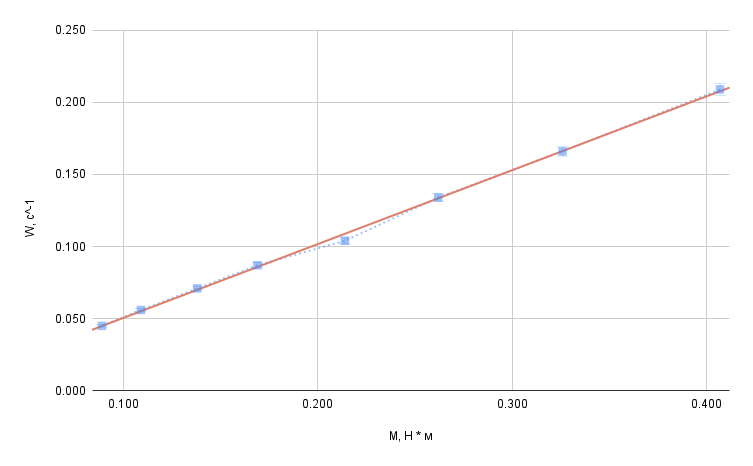
\includegraphics[scale=0.7]{chart.png}
	\caption{График зависимости скорости прецессии гироскопа от момента силы}
	\label{graph}
\end{figure}


Коэффициент $ k $ можно вычислить по следующей формуле:\label{k}

\begin{equation}
k = \frac{\langle M\Omega\rangle}{\langle M^2 \rangle} \approx 0,5122 \text{ } \frac{1}{\text{Дж} \cdot \text{с}}.
\end{equation}

Погрешность $ k $ можно вычислить следующим образом:

\begin{equation}
\sigma_k = k\sqrt{\left( \frac{\sigma_M}{M} \right)^2+\left(\frac{\sigma_\Omega}{\Omega} \right)^2} \approx 0,0054 \text{ } \frac{1}{\text{Дж} \cdot \text{с}}.
\end{equation}
В итоге: 

\bigskip
\underline{$ k =\left( 0,5122 \pm 0,0054 \right) \frac{1}{\text{Дж} \cdot \text{с}} , \left( \varepsilon = 1,0 \% \right) $} 
\bigskip

С помощью $ k $ можно вычислить угловую скорость вращения ротора гироскопа:

\begin{equation}
\omega_0 = \frac{1}{I_0 k} \approx 2535,5 \text{ с}^{-1},
\end{equation}
где $ I_0 $ -- момент инерции ротора гироскопа, вычисленный выше.

Тогда погрешность вычисления $ \omega_0 $ можно определить по формуле:

\begin{equation}
\sigma_{\omega_0} = \omega_0 \sqrt{\left( \frac{\sigma_{I_0}}{I_0} \right)^2 + \left( \frac{\sigma_k}{k} \right)^2} \approx 102,3 \text{ с}^{-1}.
\end{equation}

Таким образом, получаем:
\bigskip

	 \underline{$ \omega_0 =\left( 2535,5 \pm 102,3 \right) \text{ с}^{-1} ,  \left( \varepsilon = 4,0 \% \right) $}

\bigskip

Используя угловую скорость, можно определить частоту вращения ротора гироскопа:

\begin{equation}
\nu = \frac{\omega_0}{2\pi} \approx 403,5 \text{ Гц}.
\end{equation}

Погрешность определения частоты вращения вычисляется по следующей формуле:

\begin{equation}
\sigma_\nu = \nu \varepsilon_{\omega_0} \approx 16,3 \text{ Гц}.
\end{equation}

Таким образом, мы получили:

\bigskip
	 \underline{$ \nu = \left( 403,5 \pm 16,3 \right) \text{ Гц}, \left( 
      \varepsilon = 4,0 \% \right) $}

\bigskip
Скорость вращения ротора гироскопа можно определить и не прибегая к исследованию прецессии. У используемых в работе гироскопов статор имеет две обмотки, необходимые для быстрой раскрутки гироскопа. В данном случае одну обмотку используют для раскрутки гироскопа, а вторую -- для измерения числа оборотов ротора. Ротор электромотора всегда немного намагничен. Вращаясь, он наводит во второй обмотке переменную ЭДС индукции, частота которой равна частоте вращения ротора. Частоту этой ЭДС измеряем по фигурам Лиссажу, получаемым на экране осциллографа, если на один вход подать исследуемую ЭДС, а на другой — переменное напряжение с хорошо прокалиброванного генератора. При совпадении частот на экране получится неподвижный эллипс.\\
При настройке генератора сигнала на частоту \underline{$ \nu_0 = 392$ Гц} на экране осциллографа виден  неподвижный эллипс, следовательно эта частота сигнала совпадает с частотой вращения ротора гироскопа.


Для оценки момента силы трения, действующего на ось гироскопа, исследуем зависимость опускания оси гироскопа от времени:  $\alpha = 0,314 \ \text{рад}, \ t = 139,4 \ \text{c} $ 

\begin{equation}
M = \Omega I_0\omega_0 = \frac{\Omega}{k} \approx 3 \cdot 10^{-3} \text{ } \text{Н} \cdot \text{м},
\end{equation}

\section*{Вывод}
В ходе работы мы определили частоту вращения ротора гироскопа:

\bigskip
	$ \nu = \left( 403,5 \pm 16,3 \right) \text{ Гц}, \left( \varepsilon = 4,0 \% \right)   $
\bigskip

Полученная частота совпадает со значение частоты, измеренным с помощью осциллографа ($ \nu_\text{осц} = 392 $ Гц) в пределах погрешности.\\
Также был оценен момент силы трения, действующий на ось гироскопа $ M \approx 3 \cdot 10^{-3} \text{ } \text{Н} \cdot \text{м} $.

  
\end{center}





















\end{document}
